% Dataset Statistics Diagram
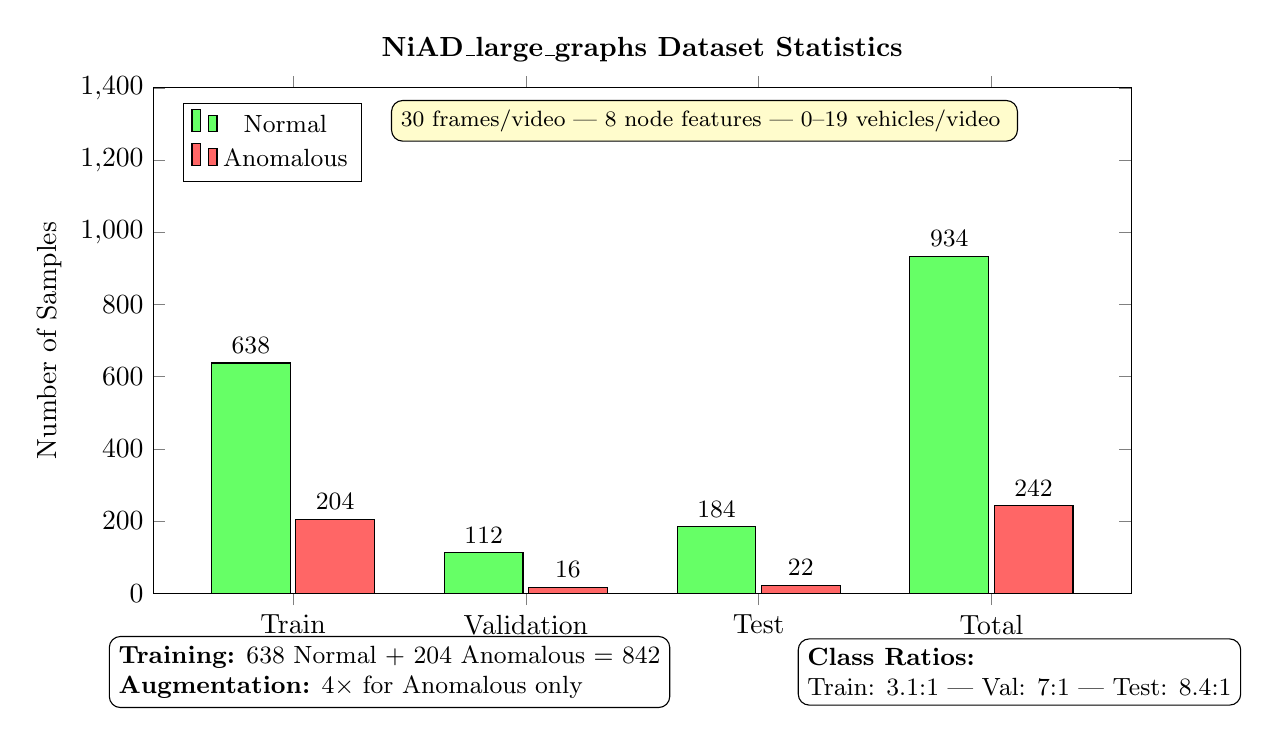
\begin{tikzpicture}
\begin{axis}[
    ybar,
    width=14cm,
    height=8cm,
    bar width=1cm,
    ylabel={Number of Samples},
    symbolic x coords={Train, Validation, Test, Total},
    xtick=data,
    ymin=0,
    ymax=1400,
    legend pos=north west,
    legend style={font=\small},
    title={\textbf{NiAD\_large\_graphs Dataset Statistics}},
    title style={font=\bfseries},
    nodes near coords,
    nodes near coords style={font=\small},
    enlarge x limits=0.2
]

% Normal class
\addplot[fill=green!60] coordinates {
    (Train, 638)
    (Validation, 112)
    (Test, 184)
    (Total, 934)
};

% Anomalous class
\addplot[fill=red!60] coordinates {
    (Train, 204)
    (Validation, 16)
    (Test, 22)
    (Total, 242)
};

\legend{Normal, Anomalous}

\end{axis}

% Annotations
\node[font=\small, align=left, fill=white, draw, rounded corners] at (3, -1) {
    \textbf{Training:} 638 Normal + 204 Anomalous = 842\\
    \textbf{Augmentation:} 4$\times$ for Anomalous only
};

\node[font=\small, align=left, fill=white, draw, rounded corners] at (11, -1) {
    \textbf{Class Ratios:}\\
    Train: 3.1:1 | Val: 7:1 | Test: 8.4:1
};

% Properties annotation
\node[font=\footnotesize, align=center, fill=yellow!20, draw, rounded corners] at (7, 6) {
    30 frames/video | 8 node features | 0--19 vehicles/video
};

\end{tikzpicture}
